\documentclass[14pt]{article}

\usepackage[T1]{fontenc}
\usepackage[utf8]{inputenc}
\usepackage[russian]{babel}

% page margin
\usepackage[top=2cm, bottom=2cm, left=2cm, right=2cm]{geometry}

% AMS packages
\usepackage{amsmath}
\usepackage{amssymb}

\newcommand{\lb}{\left(}
\newcommand{\rb}{\right)}

\newcommand{\intty}{\int\limits_{-\infty}^{\infty}}

% table/tabular packages
\usepackage{tabularx, rotating, ragged2e, booktabs, caption}
\usepackage{graphicx}
\usepackage[verbose]{placeins}
\usepackage{blindtext}
\usepackage{multicol}

\begin{document}

\subsection*{Definitions}

\begin{gather}
F \lb \omega \rb = \int\limits_{-\infty}^{\infty} f(t) \exp \lb - i \omega t \rb d t \notag \\
f(t) = F^{-1} \left[ F \lb \omega \rb \right] = \int\limits_{-\infty}^{\infty} F \lb \omega \rb \exp \lb i \omega t \rb \frac{d \omega}{2 \pi} \notag
\end{gather}


\subsection*{Convolution theorem}

\begin{gather}
	f * g = \intty g \lb t^\prime \rb f \lb t - t^\prime \rb d t^\prime = \intty g(t^\prime) \left[ \, \intty F(\omega) \exp \lb i \omega (t - t^\prime) \rb \frac{d \omega}{2 \pi} \right] d t^\prime = \intty F(\omega) \left[ \, \intty g(t^\prime) \exp \lb i \omega (t - t^\prime) \rb d t^\prime \right] \frac{d \omega}{2 \pi}  = \notag \\ 
	= \intty F(\omega) G(\omega) \exp \lb i \omega t \rb \frac{d \omega}{2 \pi} = F^{-1} \left[ F(\omega) G(\omega) \right] \notag \\
	F \left[ f * g \right] = F(\omega) G(\omega) \notag
\end{gather}


\subsection*{Correlation theorem}

\begin{gather}
	f \bigstar g = \intty \bar{f}(\tau) g(t + \tau) d \tau = \intty \left[ \, \intty \bar{F}(\omega) \exp(-i \omega \tau) \frac{d \omega}{2 \pi} \right] \left[ \, \intty G(\omega^\prime) \exp \lb i \omega^\prime ( t + \tau) \rb \frac{d \omega^\prime}{2 \pi} \right] d \tau = \notag \\
	= \intty \intty \bar{F}(\omega) G(\omega^\prime) \exp \lb i \omega^\prime t \rb \left[ \, \intty \exp \lb i \tau (\omega^\prime - \omega) \rb \frac{d \tau}{2 \pi} \right] \frac{d \omega}{2 \pi} \frac{d \omega^\prime}{2 \pi} = \intty \intty \bar{F}(\omega)G(\omega^\prime) \exp \lb i \omega^\prime t \rb  \delta \lb \omega - \omega^\prime \rb \frac{d \omega}{2 \pi} d \omega^\prime = \notag \\
	= \intty \bar{F}(\omega) G(\omega) \exp \lb i \omega t \rb \frac{d \omega}{2 \pi} = F^{-1} \left[ \bar{F}(\omega) G(\omega) \right] \notag \\
	F \left[ f \bigstar g \right] = \bar{F}(\omega) G(\omega) \notag
\end{gather}

\subsection*{Autocorrelation function and Wiener-Khintchine theorem}

\begin{gather}
C(t) = f \bigstar f = \intty \bar{f}(\tau) f(t + \tau) d \tau \notag \\
F \left[ C(t) \right] = | F (\omega) |^2 \quad \longleftrightarrow \quad \intty \intty \bar{f}(\tau) f(t + \tau) \exp \lb - i \omega t \rb d t \, d \tau = \Bigg{|} \intty f(t) \exp \lb i \omega t \rb dt \Bigg{|}^2 \notag
\end{gather}

\newpage

\subsection*{Discrete Fourier transform -- toy example}

\begin{gather}
	\begin{aligned}
		& \textup{continuous} \quad \quad \quad &X(\omega) = \intty x(t) \exp \left( - 2 \pi i \omega t \right) \notag \\
	 & \textup{discrete} \quad \quad \quad & X_k = \sum_{n = 0}^{N - 1} x_n \exp \left( - \frac{2 \pi i k n}{N} \right) \notag \\
	& \quad \quad \quad \quad \quad \quad \quad  \omega \cong \frac{k}{N}, \quad \quad n \cong t
\end{aligned}
\end{gather}

\begin{figure}[!h]
\begin{center}
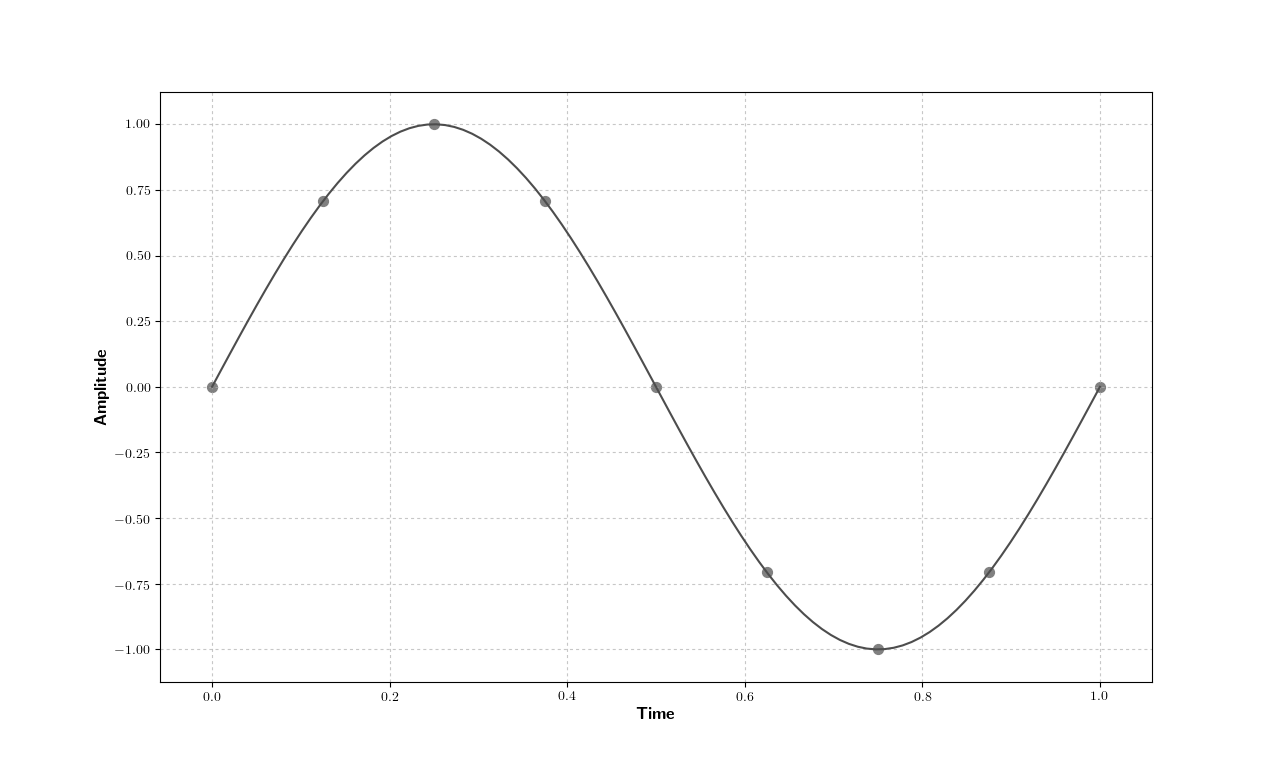
\includegraphics[width=\linewidth]{pictures/signal.png}
\end{center}
\caption{Sine wave $f(x) = \sin \lb 2 \pi x \rb$: $\omega = 1 Hz$, amplitude $ = $ 1. Sampling frequency: 8 Hz}
\end{figure}

\begin{center}
\begin{tabular}{cc}
	\toprule
	Amplitude in time domain & Amplitude in frequency domain \\
	\midrule 
	0.000 & 0.000 \\
	0.707 & -4i \\
	1.000 & 0.000 \\
	0.707 & 0.000 \\
	0.000 & 0.000 \\
       -0.707 & 0.000 \\
       -1.000 & 0.000\\
       -0.707 & 4i \\
	\bottomrule
\end{tabular}
\end{center}

Frequency resolution = $\displaystyle \frac{\textup{Sampling frequency}}{\textup{Number of samples}} = \frac{8 \textup{Hz}}{8} = 1 \textup{Hz}$. 
\begin{figure}[!h]
	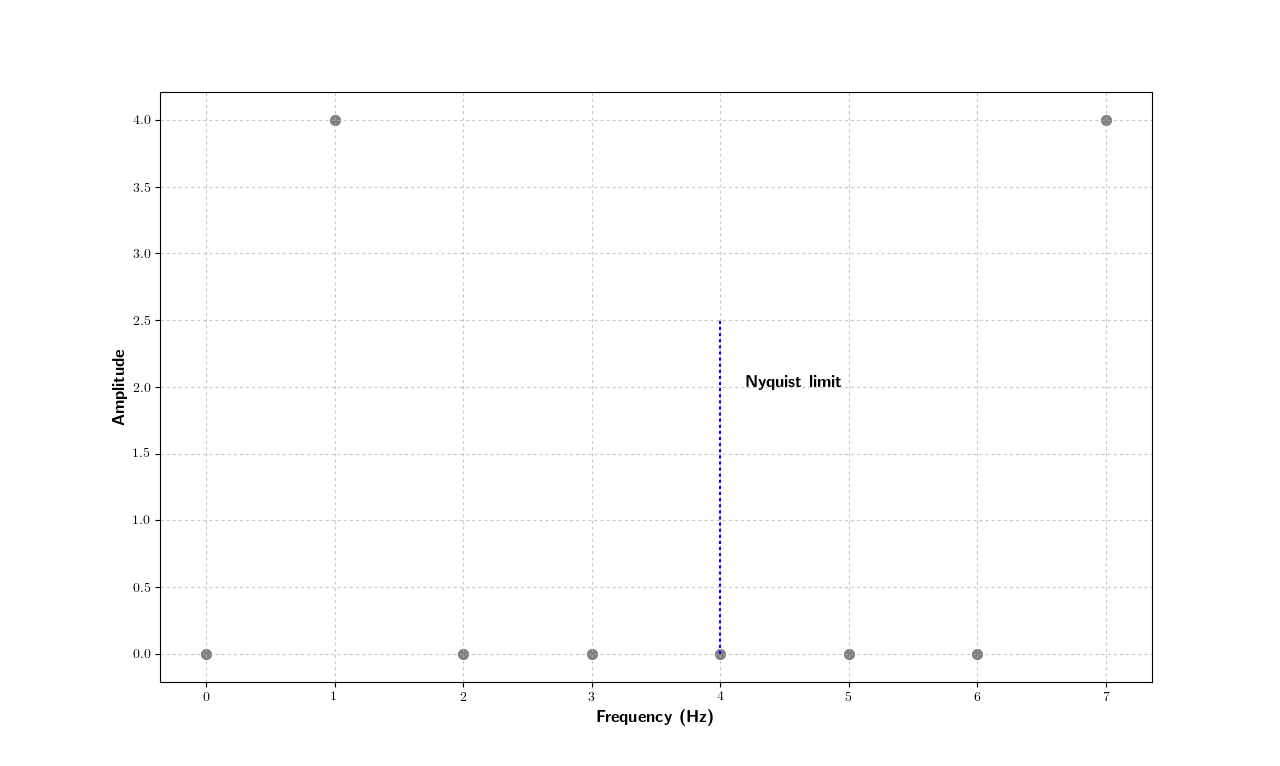
\includegraphics[width = \linewidth]{pictures/power_spectrum.png}
	\caption{Power spectrum. $\omega_i$ -- $|X_i|$.}
\end{figure}

Getting rid of all frequencies above Nyquist limit, doubling amplitudes and normalizing amplitudes by number of samples.

\begin{figure}[!h]
	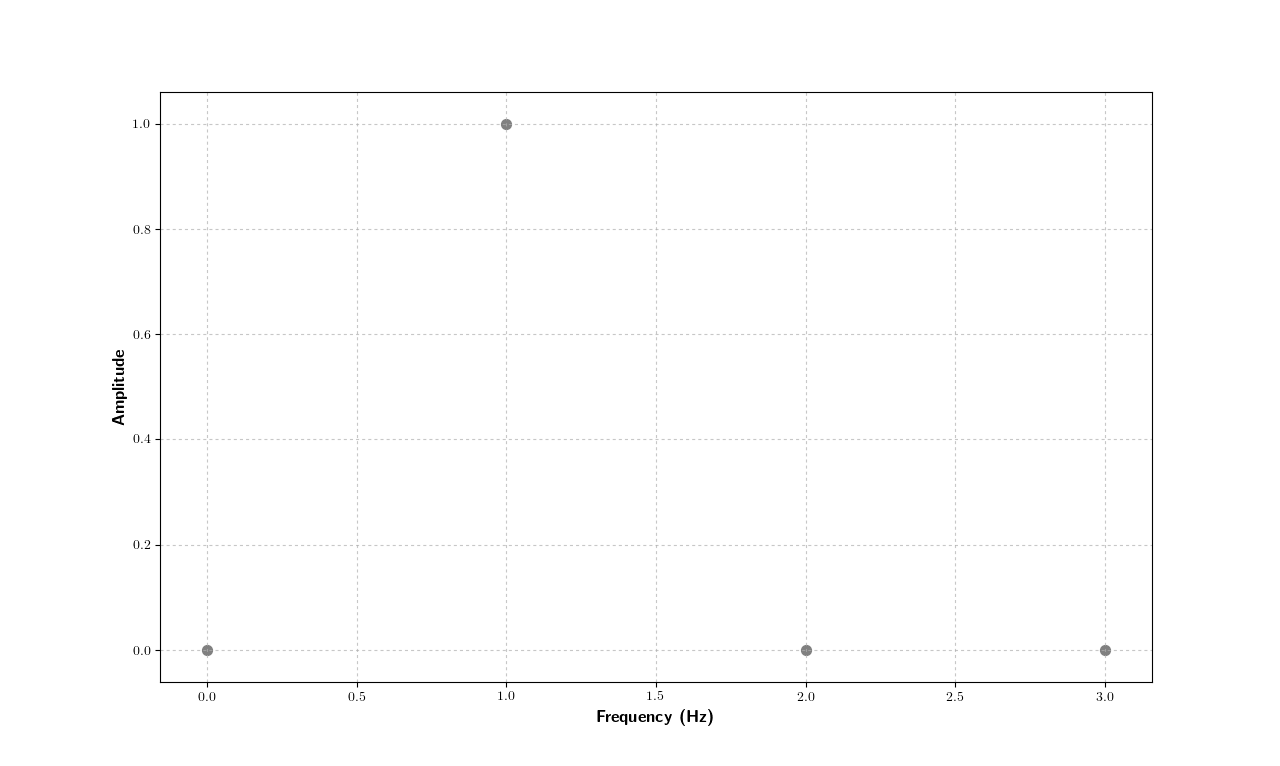
\includegraphics[width = \linewidth]{pictures/true_spectra.png}
	\caption{Normalized power spectrum}
\end{figure}

\end{document}


